%%
%% This is file `sample-sigconf.tex',
%% generated with the docstrip utility.
%%
%% The original source files were:
%%
%% samples.dtx  (with options: `all,proceedings,bibtex,sigconf')
%% 
%% IMPORTANT NOTICE:
%% 
%% For the copyright see the source file.
%% 
%% Any modified versions of this file must be renamed
%% with new filenames distinct from sample-sigconf.tex.
%% 
%% For distribution of the original source see the terms
%% for copying and modification in the file samples.dtx.
%% 
%% This generated file may be distributed as long as the
%% original source files, as listed above, are part of the
%% same distribution. (The sources need not necessarily be
%% in the same archive or directory.)
%%
%%
%% Commands for TeXCount
%TC:macro \cite [option:text,text]
%TC:macro \citep [option:text,text]
%TC:macro \citet [option:text,text]
%TC:envir table 0 1
%TC:envir table* 0 1
%TC:envir tabular [ignore] word
%TC:envir displaymath 0 word
%TC:envir math 0 word
%TC:envir comment 0 0
%%
%%
%% The first command in your LaTeX source must be the \documentclass
%% command.
%%
%% For submission and review of your manuscript please change the
%% command to \documentclass[manuscript, screen, review]{acmart}.
%%
%% When submitting camera ready or to TAPS, please change the command
%% to \documentclass[sigconf]{acmart} or whichever template is required
%% for your publication.
%%
%%
\documentclass[sigconf]{acmart}
%\documentclass[sigconf,authorversion,nonacm]{acmart}
\settopmatter{printacmref=false} 
%\settopmatter{printacmref=false} % Removes citation information below abstract
%\renewcommand\footnotetextcopyrightpermission[1]{} % removes footnote with conference information in first column
%\pagestyle{plain}

\renewcommand\footnotetextcopyrightpermission[1]{}

\usepackage{amsmath}
\usepackage{dsfont}
\usepackage{algorithmicx}
\usepackage[ruled,commentsnumbered,boxed]{algorithm2e}
\usepackage{multirow}
\usepackage{graphicx}
\usepackage{subcaption}
\usepackage{xcolor} 
\usepackage{adjustbox}



%%
%% \BibTeX command to typeset BibTeX logo in the docs
\AtBeginDocument{%
  \providecommand\BibTeX{{%
    Bib\TeX}}}

%% Rights management information.  This information is sent to you
%% when you complete the rights form.  These commands have SAMPLE
%% values in them; it is your responsibility as an author to replace
%% the commands and values with those provided to you when you
%% complete the rights form.
%\setcopyright{acmlicensed}
%\copyrightyear{2018}
%\acmYear{2018}
%\acmDOI{XXXXXXX.XXXXXXX}

%% These commands are for a PROCEEDINGS abstract or paper.
%\acmConference[Conference acronym 'XX]{Make sure to enter the correctconference title from your rights confirmation emai}{June 03--05,2018}{Woodstock, NY}
%%
%%  Uncomment \acmBooktitle if the title of the proceedings is different
%%  from ``Proceedings of ...''!
%%
%%\acmBooktitle{Woodstock '18: ACM Symposium on Neural Gaze Detection,
%%  June 03--05, 2018, Woodstock, NY}
%\acmISBN{978-1-4503-XXXX-X/18/06}


%%
%% Submission ID.
%% Use this when submitting an article to a sponsored event. You'll
%% receive a unique submission ID from the organizers
%% of the event, and this ID should be used as the parameter to this command.
%\acmSubmissionID{2718}

\acmConference[CIKM'24]{ACM Conference}{Oct 2024}{Boise, Idaho, USA}

%%
%% For managing citations, it is recommended to use bibliography
%% files in BibTeX format.
%%
%% You can then either use BibTeX with the ACM-Reference-Format style,
%% or BibLaTeX with the acmnumeric or acmauthoryear sytles, that include
%% support for advanced citation of software artefact from the
%% biblatex-software package, also separately available on CTAN.
%%
%% Look at the sample-*-biblatex.tex files for templates showcasing
%% the biblatex styles.
%%

%%
%% The majority of ACM publications use numbered citations and
%% references.  The command \citestyle{authoryear} switches to the
%% "author year" style.
%%
%% If you are preparing content for an event
%% sponsored by ACM SIGGRAPH, you must use the "author year" style of
%% citations and references.
%% Uncommenting
%% the next command will enable that style.
%%\citestyle{acmauthoryear}


%%
%% end of the preamble, start of the body of the document source.
\begin{document}

%%
%% The "title" command has an optional parameter,
%% allowing the author to define a "short title" to be used in page headers.
\title{Query-Enhanced Adaptive Semantic Path Reasoning for Inductive Knowledge Graph Completion}

%%
%% The "author" command and its associated commands are used to define
%% the authors and their affiliations.
%% Of note is the shared affiliation of the first two authors, and the
%% "authornote" and "authornotemark" commands
%% used to denote shared contribution to the research.
\author{Kai Sun}
%\authornote{Both authors contributed equally to this research.}
% \orcid{1234-5678-9012}
\affiliation{%
  \institution{Beijing University of Technology}
  \city{Beijing}
  \country{China}}
\email{sunkai@emails.bjut.edu.cn}

\author{Jiapu Wang}
\authornote{Both authors contributed equally to this research.}
\affiliation{%
  \institution{Beijing University of Technology}
  \city{Beijing}
  \country{China}}
\email{jpwang@emails.bjut.edu.cn}

\author{Huajie Jiang}
\affiliation{%
  \institution{Beijing University of Technology}
  \city{Beijing}
  \country{China}}
\email{jianghj@bjut.edu.cn}

\author{Yongli Hu}
\affiliation{%
 \institution{Beijing University of Technology}
  \city{Beijing}
  \country{China}}
\email{huyongli@bjut.edu.cn}

\author{Baocai Yin}
\affiliation{%
  \institution{Beijing University of Technology}
  \city{Beijing}
  \country{China}}
\email{ybc@bjut.edu.cn}

%
% By default, the full list of authors will be used in the page
% headers. Often, this list is too long, and will overlap
% other information printed in the page headers. This command allows
% the author to define a more concise list
% of authors' names for this purpose.
% \renewcommand{\shortauthors}{Sun et al.}
% \author{Anonymous authors}
%  \affiliation{
%    \institution{Paper under double-blind review}
%  }
\renewcommand{\shortauthors}{Sun, et al.}


%%
%% The abstract is a short summary of the work to be presented in the
%% article.
\begin{abstract}
Conventional Knowledge graph completion (KGC) methods aim to infer missing information in incomplete Knowledge Graphs (KGs) by leveraging existing information, which struggle to perform effectively in scenarios involving emerging entities.
Inductive KGC methods can handle the emerging entities and relations in KGs, offering greater dynamic adaptability. While existing inductive KGC methods have achieved some success, they also face challenges, such as susceptibility to noisy structural information during reasoning and difficulty in capturing long-range dependencies in reasoning paths. To address these challenges, this paper proposes the \textbf{Q}uery-Enhanced \textbf{A}daptive \textbf{S}emantic \textbf{P}ath \textbf{R}easoning (QASPR) framework, which simultaneously captures both the structural and semantic information of KGs to enhance the inductive KGC task. Specifically, the proposed QASPR employs a query-dependent masking module to adaptively mask noisy structural information while retaining important information closely related to the targets. Additionally, QASPR introduces a global semantic scoring module that evaluates both the individual contributions and the collective impact of nodes along the reasoning path within KGs. %This module can accurately identify critical semantic paths for effective reasoning, capturing long-range semantic dependencies in the reasoning path. 
The experimental results demonstrate that QASPR achieves state-of-the-art performance.

%Inductive knowledge graph completion (KGC) methods are ideal for evolving scenarios, where entities in the testing phase are unseen during training. Methods based on Graph Neural Networks and self-supervised learning for inductive KGC have been extensively explored and have demonstrated promising effectiveness. However, existing methods still face challenges. Firstly, the highly complex structure of knowledge graphs (KGs) introduces substantial noise, hindering the effective utilization of structural characteristics. Secondly, existing research typically focuses only on the current node in the reasoning path, overlooking long-range semantic dependencies among entities, thereby reducing the effectiveness of reasoning tasks. To address these challenges, this paper proposes the \textbf{Q}uery-Enhanced \textbf{A}daptive \textbf{S}emantic \textbf{P}ath \textbf{R}easoning (QASPR) framework. Specifically, QASPR employs a query-dependent masking mechanism to mask noisy edges adaptively, retaining edges closely related to the targets. Additionally, QASPR introduces a comprehensive path-scoring mechanism that evaluates both the individual contributions and the collective impact of nodes along the reasoning path within KGs, thereby capturing long-range semantic dependencies among entities. The experimental results demonstrate that QASPR achieves state-of-the-art performance.
\end{abstract}

%%
%% The code below is generated by the tool at http://dl.acm.org/ccs.cfm.
%% Please copy and paste the code instead of the example below.
%%
\begin{comment}
\begin{CCSXML}
<ccs2012>
 <concept>
  <concept_id>00000000.0000000.0000000</concept_id>
  <concept_desc>Do Not Use This Code, Generate the Correct Terms for Your Paper</concept_desc>
  <concept_significance>500</concept_significance>
 </concept>
 <concept>
  <concept_id>00000000.00000000.00000000</concept_id>
  <concept_desc>Do Not Use This Code, Generate the Correct Terms for Your Paper</concept_desc>
  <concept_significance>300</concept_significance>
 </concept>
 <concept>
  <concept_id>00000000.00000000.00000000</concept_id>
  <concept_desc>Do Not Use This Code, Generate the Correct Terms for Your Paper</concept_desc>
  <concept_significance>100</concept_significance>
 </concept>
 <concept>
  <concept_id>00000000.00000000.00000000</concept_id>
  <concept_desc>Do Not Use This Code, Generate the Correct Terms for Your Paper</concept_desc>
  <concept_significance>100</concept_significance>
 </concept>
</ccs2012>
\end{CCSXML}

\ccsdesc[500]{Do Not Use This Code~Generate the Correct Terms for Your Paper}
\ccsdesc[300]{Do Not Use This Code~Generate the Correct Terms for Your Paper}
\ccsdesc{Do Not Use This Code~Generate the Correct Terms for Your Paper}
\ccsdesc[100]{Do Not Use This Code~Generate the Correct Terms for Your Paper}
\end{comment}

%%
%% Keywords. The author(s) should pick words that accurately describe
%% the work being presented. Separate the keywords with commas.

\keywords{Knowledge Graph, Inductive Knowledge Graph Completion, Long-range Semantic Dependencies, Query-dependent Masking}

%% A "teaser" image appears between the author and affiliation
%% information and the body of the document, and typically spans the
%% page.

%%
%% This command processes the author and affiliation and title
%% information and builds the first part of the formatted document.
\maketitle
\section{Introduction}
Knowledge Graphs (KGs) are structured graph networks where entities are represented as nodes and relations as edges. Currently, KGs are widely used in fields such as recommendation systems \cite{wei2022contrastive} and natural language processing \cite{wang2023survey}. However, due to the continuous emergence of new knowledge, the issue of incompleteness in knowledge graphs has garnered increasing attention. To address this, the task of Knowledge Graph Completion (KGC) \cite{wang2023multi} has emerged, aiming to leverage existing knowledge to infer missing facts and enhance completeness. Although traditional KGC methods \cite{10115028, ho2018rule, wang2022multi} have made some progress, they only address entities already present in KGs and struggle to perform effectively in scenarios involving emerging entities. To tackle these issues, inductive KGC methods \cite{teru2020inductive, chen2021topology, zhu2021neural, zhang2021knowledge} have been developed. %These methods not only adapt to the continuous changes in knowledge graphs but also significantly improve completion performance, allowing for a more accurate reflection of the complexities of the real world.

%However, due to the continuous emergence of new knowledge, KGs are often incomplete, necessitating the use of Knowledge Graph Completion (KGC) methods \cite{10115028, wang2023multi} to fill in missing links and enhance the integrity of the graph. Although traditional KGC methods \cite{bordes2013translating, ho2018rule, 10132432} have made some progress, they are unable to handle new entities and often overlook the dynamic nature of KGs. To address these issues, Inductive Knowledge Graph Completion (IKGC) methods \cite{teru2020inductive, chen2021topology, zhu2021neural, zhang2021knowledge} have been developed. These methods not only adapt to the ongoing changes and expansions in KGs but also significantly improve completion performance, making the graphs more accurately reflect the complexities of the real world.

%Knowledge Graphs (KGs) represent real-world entities as nodes and the relations between them as edges, forming a structured graph of interconnected information. They are widely used in various applications, including search engines, recommendation systems, and natural language processing. Due to their ability to provide rich and semantic context, they

%Knowledge Graphs (KGs) represent real-world entities as nodes and the relations between them as edges. Knowledge Graph Completion (KGC) is designed to address the issues of incompleteness and inaccuracies in KGs. Nonetheless, prior research \cite{bordes2013translating,ho2018rule,10132432} has overlooked the evolutionary nature of KGs. To address this gap, various inductive KGC \cite{teru2020inductive,chen2021topology,zhu2021neural,zhang2021knowledge} methods have been developed, achieving notable performance improvements.

%Most previous works only consider the transductive scenario where entities are existing in KGs, which cannot work effectively for the inductive scenario containing emerging entities.

Inductive KGC typically relies on techniques such as Graph Neural Networks (GNNs) \cite{wang2022exploring, zhu2023net} and self-supervised learning \cite{9864100} to learn general representations from the graph structure and handle the introduction of new entities. Despite the progress made by current methods, they still face numerous challenges. On the one hand, as shown in Figure \ref{path}, previous research has often overlooked the significant challenges posed by the highly complex structures of KGs. The complexity of KGs, with their numerous nodes and edges representing diverse and intricate relation types, can introduce noise during the reasoning process and hinder the effective utilization of structural characteristics \cite{wang2024made}. Thus, effectively removing the noise from irrelevant structural information within KGs is crucial.
%The complex KGs contain a large number of nodes and edges with diverse and complex relation types, which may introduce noise during the reasoning process, and hinder the effective exploitation of structural characteristics. Thus, how to effective remove the noise of the irrelevant structural information within the KGs is crucial.

\begin{figure}[t]
\centering
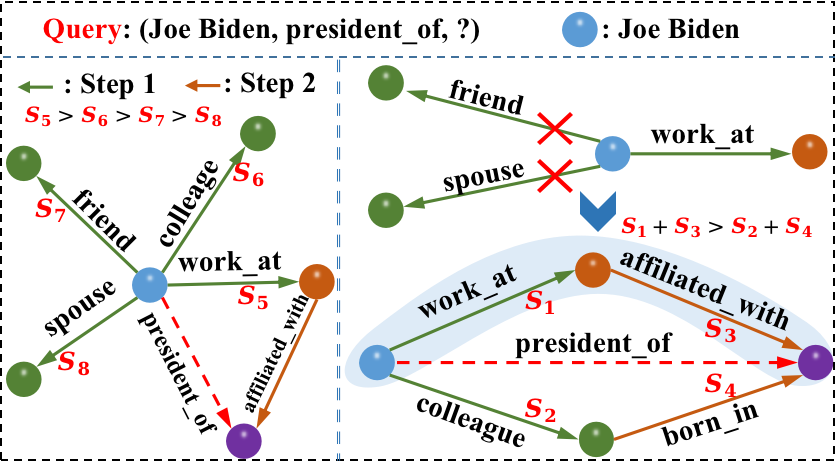
\includegraphics[scale=0.55]{Figure_path.png}
\vspace{-10pt}
\caption{The motivation of the conventional inductive KGC (left) and the proposed QASPR (right). Conventional inductive KGCs traverse nodes directly over KGs. QASPR sequentially masks the noise structure and
captures the long-range semantic dependencies over the whole reasoning path.}
\label{path}
\end{figure}

\begin{figure*}[t]
\centering

\includegraphics[scale=0.65]{framework.png}
\caption{The whole framework of QASPR.
Specifically, Query-dependent masking module adaptively masks the noisy structural information, thereby retaining effective structure; Global semantic scoring module captures the long-range dependencies by evaluating the semantics of the whole reasoning path; MLP is utilized to compute the scores for the candidates. \textbf{m} indicates the number of reasoning paths and \textbf{n} denotes number of nodes in every reasoning path.}
\label{overview}
\end{figure*}

On the other hand, prior research has typically focused only on the immediately current node in the reasoning path, overlooking the critical long-range semantic dependencies among entities throughout the entire reasoning path. %Existing methods usually emphasize the impact of the previous node, neglecting the influence of all preceding nodes along the entire reasoning path on the current node. 
This oversight can lead to an incomplete understanding of the semantic context, thereby reducing the effectiveness of reasoning tasks. Therefore, it is essential to develop a mechanism that captures the full scope of semantic dependencies, considering the cumulative influence of all nodes in the reasoning path.

%However, existing approaches overlook the significance of these extensive semantic dependencies, resulting in models that are constrained in their ability to perform deep semantic analysis.

To address these challenges, this paper proposes the \textbf{Q}uery-Enhanced \textbf{A}daptive \textbf{S}emantic \textbf{P}ath \textbf{R}easoning (QASPR) framework, which simultaneously captures both structural and semantic information of KGs to enhance the inductive KGC task. Specifically, the proposed QASPR employs a query-dependent masking module to adaptively mask the noisy edges, retaining edges closely related to the targets. Additionally, QASPR introduces a global semantic scoring module that evaluates both the individual contributions and the collective impact of nodes along the reasoning path within KGs. This module can accurately identify critical semantic paths for effective reasoning, capturing long-range semantic dependencies in the reasoning path.

%that evaluates not only the individual contributions, including influence or centrality, of each node on a path but also their synergistic effects, including enhanced connectivity or reinforced semantic relevance, within the knowledge graph. This precision enables the accurate identification of important semantic paths, thereby effectively capturing long-range semantic dependencies between entities essential for advanced reasoning tasks.

%, which enhances the reasoning process through a refined denoising approach and effectively captures long-range semantic dependencies. Specifically, the framework employs a query-dependent knowledge graph masking (KG mask) mechanism that integrates Bernoulli distribution with single rules(i.e., ordered relation pairs) to retain edges closely related to the targets selectively. Additionally, we have developed a comprehensive path-scoring mechanism that evaluates not only the individual contributions, including influence or centrality, of each node on a path but also their synergistic effects, including enhanced connectivity or reinforced semantic relevance, within the knowledge graph. This precision enables the accurate identification of important semantic paths, thereby effectively capturing long-range semantic dependencies between entities essential for advanced reasoning tasks.

To summarize, the main contributions of this paper are as follows: (1) This paper proposes a novel Query-Enhanced Adaptive Semantic Path Reasoning (QASPR) framework to capture both structural and semantic information of KGs, enhancing the inductive KGC task; (2) This paper designs a query-dependent masking module, which adaptively masks the noisy structures and retains the relevant structures within KGs in a data-driven manner; (3) This paper introduces an innovative path global semantic scoring module to capture the long-range semantic
dependencies of the reasoning path within KGs; 
%\begin{itemize}
%\item This paper proposes a novel Query-Enhanced Adaptive Semantic Path Reasoning (QASPR) framework to capture both structural and semantic information of KGs, enhancing the inductive KGC task;
%\item This paper designs a query-dependent masking module, which adaptively masks the noising structures and retains the relevant structures within KGs in a data-driven manner;
%that utilizes a combination of the Bernoulli distribution and ordered relation pairs. This module precisely filters edges that are directly relevant to specific queries, significantly enhancing the model's reasoning performance;
%\item This paper introduces an innovative path scoring module to capture the long-range semantic dependencies of the reasoning path within KGs; 

%This paper conducts extensive experiments on two benchmark datasets to evaluate the effectiveness of QASPR. 
%The experimental results demonstrate that the proposed QASPR surpasses state-of-the-art baselines in terms of prediction accuracy.
%\end{itemize}

\section{Preliminary}
\textbf{Inductive Knowledge Graph Completion}. A knowledge graph, denoted as $\mathcal{G} = (\mathcal{V}, \mathcal{E}, \mathcal{R})$, consists of finite sets of facts (edges) $\mathcal{E}$, entities (nodes) $\mathcal{V}$, and relations  $\mathcal{R}$. Each fact is represented as a triplet $(s, r, o) \in \mathcal{V} \times \mathcal{R} \times \mathcal{V}$, indicating a relation $r$ from the head entity $s$ to the tail entity $o$. KGC typically predicts the missing information through the known knowledge. Specifically, for a query $(s, r_q, ?)$, the goal is to find the set of answers $\mathcal{V}{(s,r_q,?)}$ such that for all $o \in \mathcal{V}{(s,r_q,?)}$, the triplet $(s, r_q, o)$ holds true. Based on KGC, inductive KGC is used to predict missing facts for emerging entities that never appear in KGs. %E′={(s′,q′,o′)|(s′,r′,o′)∉E,s′∈V′oro′∈V′,r′∈RwhereV′⋂V=∅andV′≠∅}\mathcal{E}' = \{(s',q',o')\\|(s',r',o') \notin \mathcal{E}, s' \in \mathcal{V}' \text{or} \; o' \in \mathcal{V}', r' \in \mathcal{R} \; where \; \mathcal{V}' \bigcap \mathcal{V} = \emptyset \; and \;  \mathcal{V}' \neq \emptyset \}.

\textbf{Logical Rules}. Logical rules $\rho$ \cite{sadeghian2019drum, wang2024large} define the relation between two entities $s$ and $o$:
\begin{equation}
\label{logical_rule}
\begin{aligned}
    \rho:\wedge_{i=1}^{l-1}r^{*}(s,o_i) \Rightarrow r_l(s,o),
\end{aligned}
\end{equation}
where the right-hand side denotes the rule head with relation $r$ that can be induced by ($\Rightarrow$) the left-hand rule body. The rule body is represented by the conjunction ($\wedge$) of a series of body relations $r^* \in \{r_1,...,r_{l-1}\}$. The logical rule is referred to as the single rule when $r^*= r_1$. 

% \textbf{Single Rule.} A single rule holds between relation r1r_1 and relation r2r_2 if ∀x,y\forall x,y:
% \vspace{-3pt}
% \begin{equation}
% \label{logical_rule}
% \begin{aligned}
%    r_{1}(x,y) \Rightarrow r_{2}(x,y),
% \end{aligned}
% \end{equation}
% where xx and yy denote the entities respectively.

\section{Method}
In this section, we introduce the Query-Enhanced Adaptive Semantic Path Reasoning (QASPR) framework for inductive KGC. QASPR mainly comprises two modules, including the query-dependent masking and global semantic scoring modules. Specifically, the query-dependent masking module employs the Bernoulli distribution \cite{zhu2021graph} to mask the noisy structures, thereby obtaining effective structural characteristics. The global semantic scoring module evaluates the semantics of the whole reasoning path to capture long-range semantic dependencies, thereby improving the accuracy of reasoning tasks. The framework is illustrated in Figure \ref{overview}.

\subsection{Query-Dependent Masking}
The query-dependent masking module utilizes the Bernoulli distribution to adaptively mask the noisy structures irrelevant to the query, thereby retaining critical structural information. Specifically, this module first extracts single rules and calculates their confidence to evaluate the relevance between relations. Subsequently, it applies a normalization strategy to convert this confidence into probability. Finally, the Bernoulli distribution is employed to filter out the irrelevant relations. %{\color{red}{This query-dependent masking module allows the model to prioritize highly relevant relations while also considering less relevant ones, thus preserving critical structural information loss and preventing overfitting.}}

Firstly, following logical notations, we denote potential relevance between relation $r$ and relation $r_q$ using a single rule $r \Rightarrow r_q$. To quantify the degree of such relevance, we define the confidence of a single rule as follows:
\vspace{-3pt}
\begin{equation}
\label{confidence}
\begin{aligned}
    \mathcal{C}(r \Rightarrow r_q) = \frac {\sum_{t \in \mathcal{E}}\mathds{1}(r \in E_{r}(t) \land r_q \in E_{r}(t))}{\sum_{t \in \mathcal{E}} \mathds{1} (r \in E_{r}(t))},\nonumber
\end{aligned}
\end{equation}
where the function $\mathds{1}(x)$ equals 1 when $x$ is true and 0 otherwise, $E_{r}$ denotes the extracted relations from the triplets. %As an empirical statistic over the entire KG, C(r⇒rq)\mathcal{C}(r \Rightarrow r_q) is larger if more triplets with relation rr also have rqr_q. 
$\mathcal{C}(r \Rightarrow r_q)$ quantifies the relevance between $r$ and $r_q$; a higher value indicates stronger relevance. 

Next, we calculate the probability based on their confidence. The probability can be obtained through a normalization step that transforms the confidence into probability:
\vspace{-5pt}
\begin{equation}
\label{relevance_prob}
\begin{aligned}
    p_{rr_q}^{(l)} = \min(\frac{\mathcal{C}_{max}^{(l)}-\mathcal{C}(r \Rightarrow r_q)}{\mathcal{C}_{max}^{(l)}-\mathcal{C}_{avg}^{(l)}} \cdot p_{e},\ p_{\tau}),\nonumber
\end{aligned}
\end{equation}
where $p_{rr_q}^{(l)}$ denotes the relevance between $r$ and $r_q$, which reflects the importance of the relation $r$, probability multiplier $p_{e}$\cite{zhu2021graph} is a hyper-parameter controlling the overall probability, $\mathcal{C}_{max}^{(l)}$ and $\mathcal{C}_{avg}^{(l)}$ represent the maximum and average values within the confidence set $\mathcal{C}^{(l)}$, and $p_{\tau}$ is a cut-off probability used to truncate probability value, as extremely low probabilities can lead to the loss of important relations.

Finally, we obtain a modified subset $\widetilde{\mathcal{R}}^{(l)}$ from the candidate relations $\hat{\mathcal{R}}^{(l)}$ with certain probabilities at the $l$-th hop:

\begin{equation}
\label{bernoulli_sample}
\begin{aligned}
  \widetilde{\mathcal{R}}^{(l)} = \{r \mid r \in \hat{\mathcal{R}}^{(l)}, Bern(p_{rr_q}^{(l)}) = 1\}\nonumber,
\end{aligned}
\end{equation}
where $\hat{\mathcal{R}}^{(l)}$ denotes the set of $l$-th order neighboring relations of entity $s$, $Bern$ represents a Bernoulli distribution, $\widetilde{\mathcal{R}}^{(l)}$ is then used as the relation set.

After obtaining the subset $\widetilde{\mathcal{R}}^{(l)}$, we can effectively mask the noisy edges, thereby providing a clean KG for the subsequent reasoning process.

\subsection{Global Semantic Scoring}
% Effective path scoring is crucial for capturing long-range semantic dependencies. Accordingly, the proposed global semantic scoring module integrates current and historical node scores to achieve precise path evaluations.
 
Global semantic scoring module aims to capture long-range semantic dependencies by calculating the semantic scores along the whole reasoning path. Specifically, as the reasoning process progresses, the module continuously integrates the `current node' and transitions the previous `current node' into `historical node'. This dynamic update mechanism not only ensures the accurate transmission of semantic information during the reasoning process but also enhances the understanding and handling of complex paths.

During the \(L\)-step reasoning process, every step of the reasoning path with length \(l\) ($0<l\leq L$) treats the node reached at the step as the current node and computes its score:
\vspace{-3pt}
\begin{equation}
\begin{split}
    S_{cur}^l=\left\{
                \begin{array}{ll}
                   0, &l=0\\
                  \mathbf{W}^{T}\mathbf{Cur}(l), &1 \leq l \leq L ,\\
                \end{array}
              \right.\nonumber
\end{split}
\end{equation}
%\begin{equation}
    %S_{cur}^l = \mathbf{W}^{T}\mathbf{Cur}(l),\nonumber
%\end{equation}
where $\mathbf{W}$ indicates the learnable parameter, $\mathbf{Cur}(l)$ is the embedding of the `current node' with the length $l$. Furthermore, the reasoning path with length $(l-1)$ $(1\leq l\leq L)$ is treated as historical nodes, and the scores can be computed as follows:
\begin{equation}
\begin{split}
    S(P_{0 \rightarrow(l-1)})=\left\{
                \begin{array}{ll}
                   0, &l=1\\
                  \sum_{i\in\{1,\ l-1\}} S_{cur}^{i}, &2 \leq l \leq L ,\\
                \end{array}
              \right.\nonumber
\end{split}
\end{equation}
where $ S_{cur}^{l-1}$ represents the score of the historical node with length $(l-1)$, and $S(P_{0 \rightarrow(l-1)})$ denotes the whole score of all historical nodes.

The global semantic scoring module treats all nodes as integral components of the reasoning path. Consequently, the path score is based on the relevance of all nodes along the reasoning path, providing a more thorough assessment compared to methods that focus solely on the current node. The detail is shown as follows:
% \begin{equation}
% \label{scoring_mechanism}
% S(\mathcal{P}_{0 \rightarrow l}) =
% \sum_{\{1,\ l\}} \left(S(\mathcal{P}_{0 \rightarrow(l-1)})+ S_{cur}^l\right),\nonumber
% \end{equation}
\vspace{-3pt}
\begin{equation}
\label{scoring_mechanism}
S(P_{0 \rightarrow l}) =
S(P_{0 \rightarrow(l-1)})+ S_{cur}^l,\nonumber
\end{equation}
where $S(P_{0 \rightarrow l})$ indicates the score of the whole reasoning path with length $l$. 

\subsection{Entity Embedding} 
Entity embedding module aims to leverage the existing information in KGs to generate embeddings for emerging entities. Specifically, we first employ the global semantic scoring module to obtain the scores of various reasoning paths. Subsequently, we utilize the greedy algorithm to select the \textit{Top}-$k$ paths with the highest scores. Finally, we perform entity embedding for the emerging entities through an iterative learning strategy based on these paths.

%Entity embedding encapsulates the rich semantics of entities, which are beneficial for inductive KGC. Consequently, we begin by reviewing path-based approaches and identify their significant computational complexity as a primary limitation. Building on this analysis, we employ a greedy algorithm to effectively address this challenge. Finally, we utilize an iterative learning strategy to acquire precise embeddings for the entities.

Previous research mainly employs path-based approaches \cite{sadeghian2019drum, zhu2021neural} to obtain embeddings for emerging entities by analyzing the paths between a pair of entities within a KG \cite{wang2024large}. From a representation learning perspective, they aim to learn a representation $\mathbf{h}_{o}$ to predict the triplet $(s, r_q, o)$ based on the set of reasoning paths $\mathcal{P}$ from entity $s$ to entity $o$:
\vspace{-3pt}
\begin{equation}
\label{triple_embd}
\begin{aligned}
    \mathbf{h}_{o} = \sum_{P \in \mathcal{P}}\sum _{(u,r,v)\in P} \mathbf{h}_{(u,r,v)} = \sum_{P \in \mathcal{P}}\sum _{(u,r,v)\in P} \mathbf{W}_{r_q}^{T}[\mathbf{h}_{r_q};\mathbf{h}_{r}],
\end{aligned}
\end{equation}
where $[\cdot;\cdot]$ is the concatenation operator, $\mathbf{h}_{(u,r,v)}$ is the representation of triplet $(u, r, v)$  based on the query relation $r_q$, $\mathbf{W}_{r_q}$ is a learnable parameter, $\mathbf{h}_{r_q}$ denotes the representation of the relation $r_q$, and $\mathbf{h}_{r}$ denotes the representation of the relation $r$.
% \textbf{Iteratively Learning.} In order to efficiently acquire the representation of triplet (s,q,t)(s, q, t), we utilize an iterative learning scheme. Specifically, within the LL-step reasoning framework, the representation at the ll-th step for each triplet (s,q,t)∈E(s, q, t) \in \mathcal{E} is derived by combining the representation from the preceding step (l−1)(l-1)-th with the representation of neighboring triplets containing entity tt. This iterative learning methodology facilitates a step-by-step refinement of the triplet (s,q,t)(s, q, t) representation, contributing to a nuanced understanding of relations and semantic nuances among entities. Then Eq ref{triple_embd} is modified as follows: 

% \begin{equation}
% \label{iterative_embed}
% \mathbf{h}_{(s,q)}^{(l)}(t) =
% \begin{cases}
% \sum\limits_{i=1}^{2|\mathcal{R}|+1}\mathds{I}(\mathbf{w}_{q}(s,r_{i},t)|(s,r_{i},t) \in \mathcal{E}), & \text{if } l=1 \\
% \sum\limits_{(x,r)\in N_{er}^{(1)}(t)} (\mathbf{h}_{(s,q)}^{(l-1)}(x) + \mathbf{w}_{q}(x,r,t)), & \text{if } 2 \leq l \leq L
% \end{cases}
% \end{equation}

% where \mathdsI(w|C)\mathds{I}(\mathbf{w}|C) is a function that returns w\mathbf{w} if CC is true or 0\mathbf{0} otherwise, rir_{i} denotes the ii-th relation and N(l)er(t)N_{er}^{(l)}(t) represents the set of ll-th order neighboring entities and relations for entity tt.
% To reduce computational complexity, we utilize a greedy algorithm capable of efficiently calculating entity embeddings. Additionally, an iterative learning strategy is deployed to enhance the accuracy of the triplets (s,rq,o)(s,r_q,o) representations through successive refinements.

It is worth noting that there are multiple paths to reach the target entity within KGs. %, and exploring a vast path space poses a significant computational challenge for the model. %For reasoning paths of length LL, there are |R|L|\mathcal{R}|^L candidate paths, which markedly amplify the computational complexity. Consequently, we modify Eq ref{iterative_embed} as follows: 
Therefore, we employ a greedy algorithm to select the \textit{Top}-$k$ paths with the highest scores:% and return the end entities associated with these paths.

\begin{equation}
\label{top_k_nodes}
\begin{aligned}
  \hat{\mathcal{V}}^{(l-1)} = Top\_k (\bigcup_{P \in \mathcal{P}_{0 \rightarrow (l-1)}} S(P_{0 \rightarrow (l-1)})),\nonumber
\end{aligned}
\end{equation}
where $\mathcal{P}_{0 \rightarrow (l-1)}$ denotes all the reasoning paths of the length $(l-1)$, $\hat{\mathcal{V}}^{(l-1)}$ denotes the set of the end entities inferred from $\mathcal{P}_{0 \rightarrow (l-1)}$.
Finally, due to the impacts of the $Top\_k$ strategy adopted by the greedy algorithm on entity embedding, we further revise Eq (\ref{triple_embd}) as follows:

% \begin{equation}
% \label{modify_scoring_mechanism}
% S(\mathcal{P}_{s \rightarrow t}^{(l)}) =
% \displaystyle \sum\limits_{\substack{(x,r)\in N_{er}^{(1)}(t)\\ x \in \hat{\mathcal{V}}^(l-1),r \in \widetilde{\mathcal{R}}^{(l)}}} \left(S(\mathcal{P}_{s \rightarrow x}^{(l-1)})+Cur(t)\right), \text{if } 1 \leq l \leq L-1
% \end{equation}
\vspace{-10pt}
\begin{equation}
\begin{split}
\mathbf{h}_{o}^{(l)} = 
\begin{cases}
\sum\limits_{\substack{(s,r,o) \in \mathcal{E}}}\mathbf{W}_{r_q}^{T}[\mathbf{h}_{r_q};\mathbf{h}_{r}], &l=1 \\
\sum\limits_{\substack{x \in \hat{\mathcal{V}}^{(l-1)}}}\sum\limits_{(x,r,o) \in \mathcal{E}} \left( \mathbf{h}_{x}^{(l-1)}+ \mathbf{W}_{r_q}^{T}[\mathbf{h}_{r_q};\mathbf{h}_{r}] \right), &2 \leq l \leq L.\nonumber
\end{cases}
\end{split}
\label{iterative_embed_for_important_path}
\end{equation}

After the above operations, we can obtain the final embedding of the predicated entity $o$.

\subsection{Loss function} \label{subsec:loss_function}
Following the strategy \cite{lacroix2018canonical}, we train the proposed QASPR through the multi-class log-loss function $\mathcal{L}$:

\begin{equation}
\label{multi-class}
    \mathcal{L} = \sum_{(s,r_q,o) \in \mathcal{E}_{train}}( -\mathbf{W}_{s}^{T}\mathbf{h}_{o}^{(L)} + \log(\sum_{\forall {x \in \mathcal{V}}}\exp(\mathbf{W}_{s}^{T}\mathbf{h}_{x}^{(L)}))),\nonumber
\end{equation}
%\vspace{-3pt}
%\begin{equation}
%\label{scorce}
    %f(s, r_q, o) = \mathbf{w}_{s}^{T}\mathbf{h}_{o}^{(L)},
%\end{equation}
where $\mathbf{W}_{s} \in \mathbb{R}^{d}$ is a weight parameter, $\mathbf{h}_{o}^{(L)}$ represents the embedding of entity $o$ at step $L$, $\mathbf{h}_{x}^{(L)}$ represents the embedding of entity $x$ at step $L$, $\mathcal{E}_{train}$ denotes the set of the positive triplets $(s,r_q,o)$.

\section{Experiments}\label{Sec:Experiments}
\subsection{Experiment setup}
In this subsection, we will outline the experimental setup for the proposed QASPR framework, detailing the datasets, baselines, and parameter settings.

\textbf{Datasets.} Based on the approach in \cite{zhu2023net}, we utilize the same subsets of WN18RR and FB15k237, with each dataset having four different versions, resulting in a total of eight subsets. Each subset includes a different split of the training set and test set. For detailed statistics, please refer to \cite{zhu2023net}.

\textbf{Baselines.} The proposed QASPR is compared with several classic inductive KGC methods, including: RuleN \cite{meilicke2018fine}, NeuralLP \cite{yang2017differentiable}, DRUM \cite{sadeghian2019drum}, GraIL \cite{teru2020inductive}, NBFNet \cite{zhu2021neural}, RED-GNN \cite{zhang2021knowledge}, AdaProp \cite{zhang2023adaprop}, A*Net \cite{zhu2023net}, and MLSAA \cite{skMLSAA2024}.

\textbf{Parameter Setting.} The proposed QASPR chooses \textit{Mean Reciprocal Rank} (MRR) \cite{wang2023multi} as evaluation metric. Additionally, we adopt Adam\cite{kingma2014adam} as the optimizer. %, and the batch size is set to 100100 across all datasets. 
%We tune the learning rate within the range of [10−4,10−2][10^{-4}, 10^{-2}] for different datasets. We perform hyperparameter tuning on a variety of settings, including weight decay within the range of [10−5,10−2][10^{-5}, 10^{-2}], layer LL chosen from {3,4,5,6,7}\{3, 4, 5, 6, 7\}, the number of sampled entities KK among {50,100,150,200,250,300}\{50, 100, 150, 200, 250, 300\}, probability multiplier pep_e chosen from {0.3,0.4,0.5,0.6,0.7,0.8}\{0.3, 0.4, 0.5, 0.6, 0.7, 0.8\} and cut-off probability pτp_\tau chosen from {0.1,0.2,0.3,0.4,0.5}\{0.1, 0.2, 0.3, 0.4, 0.5\}. 
Furthermore, we tune the length of reasoning path $L$, the number of selected paths $K$ in entity embeddings,  probability multiplier $p_e$, cut-off probability $p_{\tau}$ in query-dependent masking module, and list the detailed information of the hyper-parameter in Table \ref{inductive_setting}.
%Please refer to the table 2 for more detailed information. The whole experiment is implemented on an NVIDIA RTX 3090 GPU with i9-10900X CPU.
\vspace{-5pt}
{\small
\begin{table}[h]
\centering
\caption{Hyper-parameter configurations of QASPR on both datasets.}
\vspace{-10pt}
\label{inductive_setting}
\begin{tabular}{c@{\hspace{9pt}}c@{\hspace{9pt}}c@{\hspace{9pt}}c@{\hspace{9pt}}c@{\hspace{9pt}}c@{\hspace{9pt}}c@{\hspace{9pt}}c@{\hspace{9pt}}c}
\hline
\multirow{2}{*}{Hyper-parameters} & \multicolumn{4}{c}{WN18RR} & \multicolumn{4}{c}{FB15k237} \\
\cmidrule(lr){2-5} \cmidrule(lr){6-9}
& V1 & V2 & V3 & V4 & V1 & V2 & V3 & V4 \\
\hline
$L$ & 3 & 3 & 7 & 3 & 7 & 3 & 7 & 5 \\
$K$ & 150 & 50 & 100 & 300 & 300 & 250 & 300 & 300 \\
$p_{e}$ & 0.5 & 0.3 & 0.3 & 0.6 & 0.3 & 0.7 & 0.3 & 0.4 \\
$p_{\tau}$ & 0.5 & 0.5 & 0.5 & 0.5 & 0.5 & 0.5 & 0.5 & 0.5 \\
batch size & 100 & 50 & 100 & 10 & 20 & 10 & 20 & 20 \\
\hline
\end{tabular}
\end{table}}
\subsection{Experimental Analysis} 
As shown in Table \ref{tab:results}, the experimental results validate the superiority of the proposed QASPR method compared to the current state-of-the-art baseline methods. Our method significantly improves the performance of MRR on most datasets. This indicates that QASPR can effectively mask the noisy structural information and capture long-range semantic dependencies within KGs through the query-dependent masking and global semantic scoring module, further enhancing inductive reasoning capabilities.

AdaProp\cite{zhang2023adaprop} and A*Net\cite{zhu2023net} are two important baselines, as they both facilitate the reasoning process by capturing the structural information within KGs. However, the proposed QASPR still can obtain the significant improvements on both datasets. This phenomenon demonstrates that the query-dependent masking module can effectively mask the noisy structures, thereby enhancing the inductive KGC tasks.

%However, they overlook the impacts of noisy structures and fail to capture long-distance dependencies between entities. Consequently, experimental results demonstrate that the query-dependent masking mechanism and the global semantic scoring mechanism effectively address these issues.

{\small
\begin{table}[hthp]
\centering
\caption{Performance of inductive KGC on MRR.The best score is in bold, and the second-best score is in underlined.}
\label{tab:results}
\resizebox{\columnwidth}{!}{% 调整表格以适应单栏宽度
\begin{tabular}{lcccccccc}
\toprule
\multirow{2}{*}{Methods} & \multicolumn{4}{c}{WN18RR} & \multicolumn{4}{c}{FB15k237} \\
\cmidrule(lr){2-5} \cmidrule(lr){6-9}
& v1 & v2 & v3 & v4 & v1 & v2 & v3 & v4 \\
\midrule
RuleN & 66.8 & 64.5 & 36.8 &  62.4 & 36.3 & 43.3 & 43.9 & 42.9  \\
NeuralLP & 64.9 & 63.5 & 36.1 & 62.8 & 32.5 & 38.9 & 40.0 &  39.6 \\
DRUM & 66.6 & 64.6 & 38.0 & 62.7 & 33.3 & 39.5 & 40.2 & 41.0 \\
\cline{1-9}
GraIL & 62.7 & 62.5 & 32.3 & 55.3 & 27.9 & 27.6 & 25.1 & 22.7  \\
NBFNet & 68.4 & 65.2 & 42.5 & 60.4 & 30.7 & 36.9 & 33.1 & 30.5 \\
RED-GNN & 70.1 & 69.0 & 42.7 & 65.1 & 36.9 & 46.9 & 44.5 &  44.2\\
MLSAA & 71.6 & 70.0 & 44.8 & 65.4 & 36.8 & 45.7 & 44.2 & 43.1 \\
AdaProp & \underline{73.3} & \underline{71.5} & \underline{47.4} & \underline{66.2} & 31.0 & 47.1 & 47.1 &  45.4\\
A*Net & 72.7 & 70.4 & 44.1 & 66.1 & 45.7 & \textbf{51.0} & 47.6 & \textbf{46.6} \\
\cline{1-9}
QASPR & \textbf{79.4} & \textbf{79.8} & \textbf{52.0} & \textbf{76.4} & \textbf{48.8} & \underline{49.7} & \textbf{48.8} & \underline{46.3} \\
\bottomrule
\end{tabular}
}
\end{table}}


\subsection{Ablation Experiments}\label{subsec:ablation_studies}
%\textbf{Impact of different modules.} 
In order to analyze the impact of each module, we conduct ablation experiments to validate the effectiveness of different modules. The experimental results are shown in Table \ref{Variants}. "QASPR w/o M" means removing the query-dependent masking module, and "QASPR w/o S" means removing the global semantic scoring module. The experimental results show that our proposed QASPR has a significant improvement on both datasets. We conclude that the query-dependent masking module can effectively eliminate the interference of noisy structures, and the global semantic scoring module can fully capture long-range semantic dependencies within the whole reasoning path. %The collaboration of these two mechanisms enhances generalization and robustness.
{\small
\begin{table}[h]
\centering
\caption{Ablation studies on both datasets. "QASPR w/o M" denotes the model without query-dependent masking module. "QASPR w/o S" denotes the model without the global semantic scoring.}
\vspace{-5pt}
\label{Variants}
\resizebox{\columnwidth}{!}{% 调整表格以适应列宽
\setlength{\tabcolsep}{6pt} % 调整列间的水平填充
\begin{tabular}{lcccccc}
\toprule
\multirow{2}{*}{Methods} & \multicolumn{3}{c}{WN18RR(V4)} & \multicolumn{3}{c}{FB15k237(V4)} \\
\cmidrule(lr){2-4} \cmidrule(lr){5-7}
& MRR & H@1 & H@10 & MRR & H@1 & H@10 \\
\midrule
QASPR w/o M & 73.3 & 62.9 & 94.4 & 45.2 & 35.2 & 63.4 \\
QASPR w/o S & 76.2 & 66.7 & 95.4 & 44.6 & 34.5 & 61.8 \\
QASPR & \textbf{76.4} & \textbf{67.2} & \textbf{95.6} & \textbf{46.3} & \textbf{36.1} & \textbf{64.5} \\
\bottomrule
\end{tabular}
}
\end{table}}

\begin{figure}[h]
\centering
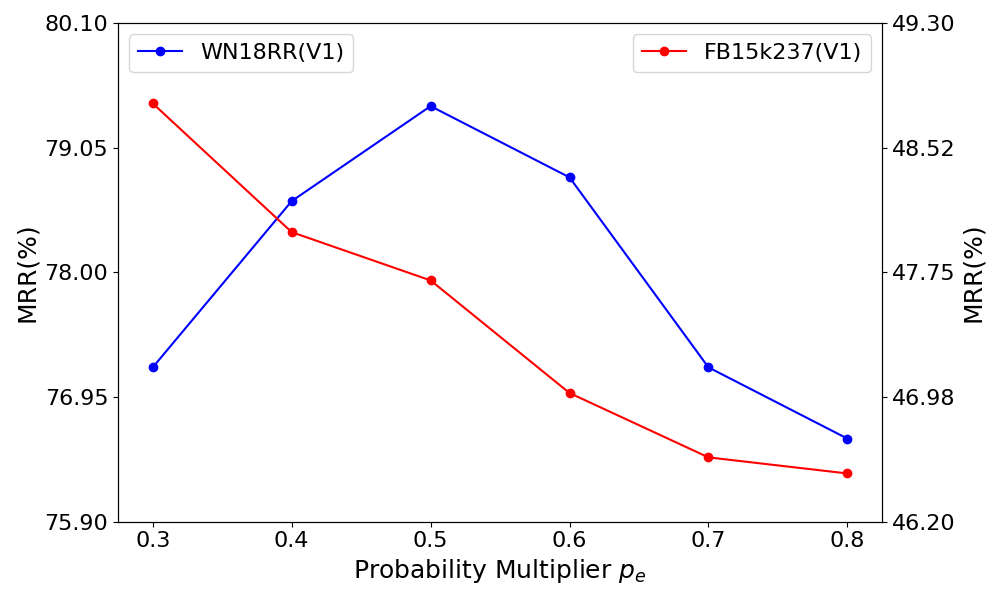
\includegraphics[scale=0.3]{pm.png}
\vspace{-10pt}
\caption{The performance with different $p_{e}$ values on WN18RR(V1) and FB15k237(V1).}
\label{pm}
\end{figure}
\subsection{Probability Multiplier $p_{e}$}
Figure \ref{pm} illustrates the trend of MRR performance for two datasets with different probability multiplier $p_e$. Overall, the MRR for the WN18RR(V1) dataset first increases and then decreases, showing a clear peak trend. In contrast, the MRR for the FB15k237(V1) dataset exhibits a continuous downward trend, with performance gradually weakening as the probability multiplier increases. This reflects the differences in how different datasets handle noise and related information. The WN18RR(V1) dataset achieves optimal performance within an intermediate range, while the FB15k237(V1) dataset shows a negative correlation with increasing probability multipliers. Therefore, selecting an optimal value of $p_e$ is crucial for maintaining model performance.

\section{Conclusion}\label{Sec:CONCLUSION}
This paper proposes a novel \textbf{Q}uery-Enhanced \textbf{A}daptive \textbf{S}emantic \textbf{P}ath \textbf{R}easoning (QASPR) framework for inductive KGC tasks. Specifically, QASPR first designs a query-dependent masking module to adaptively mask the noisy structural information, ensuring the preservation of critical information. Subsequently, QASPR develops a global semantic scoring module to capture long-range semantic dependencies in the reasoning path by evaluating the contributions of the current and historical nodes. Experimental results on two widely used datasets show the superiority of QASPR for inductive KGC tasks. 


% \begin{credits}
% % \subsubsection{\ackname} This research is supported by the National Key R\&D Program of China under Grant No.2021ZD0111902; National Natural Science Foundation of China under Grant No.U21B2038, U19B2039, 62172023 and 62206007; R\&D Program of Beijing Municipal Education Commission KZ202210005008, Beijing Natural Science Foundation 4222021, and Engineering Research Center of Intelligent Perception and Autonomous Control, Ministry of Education.
% \end{credits}
%
% ---- Bibliography ----
%
% BibTeX users should specify bibliography style 'splncs04'.
% References will then be sorted and formatted in the correct style.
%


%%
%% The acknowledgments section is defined using the "acks" environment
%% (and NOT an unnumbered section). This ensures the proper
%% identification of the section in the article metadata, and the
%% consistent spelling of the heading.

%%
%% The next two lines define the bibliography style to be used, and
%% the bibliography file.

\balance
\bibliographystyle{unsrt}
\bibliography{sample-base}

%%
%% If your work has an appendix, this is the place to put it.
\appendix
\end{document}
\endinput
%%
%% End of file `sample-sigconf.tex'.
